\documentclass[11pt,twocolumn]{article}
\usepackage[margin=1in]{geometry}
\usepackage{graphicx}
\usepackage{booktabs}
\usepackage{amsmath}
\usepackage{hyperref}
\usepackage{microtype}
\usepackage{caption}
\usepackage{subcaption}
\usepackage{listings}
\usepackage{xcolor}
\usepackage{enumitem}
\usepackage{cite}

\lstset{
  basicstyle=\ttfamily\small,
  keywordstyle=\color{blue},
  commentstyle=\color{gray},
  breaklines=true,
  frame=single,
  language=C++
}

\title{\textbf{Parallelizing Monte Carlo Value-at-Risk on a\\
       Realistic QuantLib Portfolio with OpenMP}}
\author{Muhammad Farhan\\
        \small Department of Computer Science and Engineering\\
        \small \texttt{muhammad.farhan354@gmail.com}}
\date{April 2026}

\begin{document}
\maketitle

%% ============================================================
\begin{abstract}
We parallelize the outer scenario loop of a Monte Carlo
Value-at-Risk (VaR) and Expected Shortfall (ES) engine built on the
QuantLib C++ library.  The portfolio consists of 180 instruments
(100~fixed-rate bonds, 50~interest-rate swaps, 20~European options,
10~American options priced by a 50{\texttimes}50 finite-difference
solver) repriced under 10\,000 three-factor Normal scenarios.
We introduce \texttt{ScenarioEvaluator}, a new class inside
\texttt{ql/experimental/risk/}, which pre-builds one independent
market-data and instrument clone per thread and dispatches a
\texttt{\#pragma omp parallel for} over scenarios.
Stage-by-stage profiling confirms that portfolio revaluation accounts
for 99.997\% of runtime, justifying the parallelization axis.
On a 4-socket, 64-core AMD Opteron 6272 server we achieve
\textbf{7.1$\times$} speedup at 8 threads (89\% efficiency) and
\textbf{32$\times$} at 64 threads (50\% efficiency, memory-bound).
\texttt{schedule(dynamic, 4)} outperforms \texttt{schedule(static)}
by 21\% due to scenario-dependent cost variation in the
finite-difference American option pricer.
All parallel VaR/ES values are bit-identical to the sequential
baseline.
\end{abstract}

%% ============================================================
\section{Introduction}

Portfolio Value-at-Risk and Expected Shortfall are the principal
market-risk measures mandated by the Basel~III framework and the
Fundamental Review of the Trading Book (FRTB-IMA)~\cite{bcbs2019}.
Under the internal-models approach a bank must revalue its entire
trading book under at least 10\,000 stressed historical or Monte Carlo
scenarios every business day; for large institutions with hundreds of
thousands of positions, this revaluation alone can consume several
hours of compute time.

The dominant cost is instrument repricing: each scenario requires
evaluating the pricing partial-differential equation (PDE) or
simulation for every derivative in the book.  This is an
embarrassingly parallel problem at the scenario level, yet
production systems often exploit parallelism only through coarse-grained
grid dispatch~\cite{fusai2006}, leaving intra-node CPU multicore
resources underutilised.

Contemporary work has moved toward GPU acceleration~\cite{dixon2011,
dessain2024} and multilevel stochastic approximation to reduce the
asymptotic complexity of ES estimation~\cite{crepey2025}.  However,
up-to-date empirical studies of \emph{CPU multicore} scaling on a
realistic, heterogeneous QuantLib portfolio are lacking.
This paper fills that gap: we instrument a production-representative
mixed book in QuantLib, profile the hot path, implement a
thread-safe OpenMP engine as a first-class library class, and
report scaling results across the full thread-count range of a
64-core server.

%% ============================================================
\section{Literature Survey}

\paragraph{Monte Carlo VaR complexity.}
Cr{\'e}pey et al.~\cite{crepey2025} show that standard single-level MC
achieves $O(\varepsilon^{-2})$ bias convergence for VaR but the nested
MC approach for ES degrades to $O(\varepsilon^{-3})$; their multilevel
stochastic approximation closes this to
$O(\varepsilon^{-2}|\ln\varepsilon|^2)$.
Our engine uses single-level MC
($O(1/\sqrt{N})$ convergence confirmed in E1), which is the regulatory
standard; the MLSA gap motivates future work.

\paragraph{American option parallelism.}
Bouchhima et al.~\cite{bouchhima2024} demonstrate parallel MC for
American options with CCR using the Stochastic Grid Bundling Method
on GPUs.  Our portfolio's 10 American options are priced with a
finite-difference Black--Scholes solver --- slower than
analytic methods but free of stochastic noise, making repricing
cost deterministic modulo scenario parameters.

\paragraph{GPU MC-VaR.}
Dixon et al.~\cite{dixon2011} identify three pipeline stages in a
GPU MC-VaR system: (a)~RNG and scenario generation,
(b)~distribution transform, and (c)~portfolio loss calculation via
Cholesky-decomposed factor shocks.
We adopt this decomposition to instrument stage-by-stage timing
(Section~\ref{sec:experiments}, E2) and confirm that stage~(c)
accounts for 99.997\% of sequential runtime, validating
the scenario-parallel axis.

\paragraph{QuantLib thread safety.}
Spanderen~\cite{spanderen2013} identifies the key thread-safety
hazards in QuantLib: the non-thread-safe observer/notification pattern
and the \texttt{Settings::evaluationDate()} global singleton.
He recommends either the \texttt{QL\_ENABLE\_SESSIONS} compile flag
(makes Settings thread-local) or per-thread independent market-data
views.  We implement the latter: each OpenMP thread owns a complete
independent clone of the market-data graph and instrument book, trading
memory ($64\times180$ instrument copies) for zero build-flag
dependency.

\paragraph{Parallel RNG.}
Salmon et al.~\cite{salmon2011} introduce counter-based PRNGs
(Philox, Threefry) that are stateless and reproducible across any
thread count, and pass the full TestU01 BigCrush suite.
Our V1 generates all scenarios sequentially with a single
MT19937\_64 (seed~42), which is correct and reproducible because
the pre-built scenario array is read-only during the parallel
revaluation.  Philox would be necessary if scenarios were
generated inside the parallel region.

\paragraph{Closest architectural precedent.}
Fusai et al.~\cite{fusai2006} parallelize full-revaluation VaR on a
heterogeneous 200-asset book (bonds and exotic equity derivatives)
across a 13-node grid using master--worker thread pools with adaptive
workload sizing.  Our \texttt{ScenarioEvaluator} implements the same
scenario-parallel architecture with \texttt{schedule(dynamic)}
playing the role of the adaptive workload allocator.

%% ============================================================
\section{Proposed Idea}
\label{sec:proposed}

\subsection{Architecture}

Figure~\ref{fig:pipeline} shows the pipeline.
\begin{figure}[h]
\centering
\begin{verbatim}
 Base market --> Scenario gen --> [parallel]
 (FlatForward,    (MT19937,      for s in 0..N:
  BS process)      N(0,s^2))      shockFn(ctx[tid], s)
                                  pnl[s] = sum(DNPV)
                               --> VaR/ES (sort)
\end{verbatim}
\caption{MC-VaR pipeline.  Only the revaluation loop is parallelized.}
\label{fig:pipeline}
\end{figure}

The key design component is the \texttt{ScenarioEvaluator} class
in \texttt{ql/experimental/risk/}.
Its constructor calls a user-supplied \emph{factory} once per
thread to build a \texttt{ScenarioThreadContext} --- an independent
market-data graph (SimpleQuotes, FlatForward curve, BlackConstantVol
surface) and a fully instantiated instrument book.
The \texttt{run()} method dispatches:

\begin{lstlisting}
#pragma omp parallel for
  num_threads(nt)
  schedule(dynamic, cs)
for (int s = 0; s < N; ++s) {
  int tid = omp_get_thread_num();
  shockFn(ctx[tid], s);       // shock quotes
  Real v = 0;
  for (auto& inst : ctx[tid].instruments)
    v += inst->NPV() - base[i];
  pnl[s] = v;
}
\end{lstlisting}

\noindent
The \texttt{shockFn} lambda (supplied by the driver) sets
\texttt{SimpleQuote::setValue()} on the three risk-factor quotes;
because each thread has its own quotes, there are no data races.

\subsection{Thread-safety hazards and mitigations}

\begin{itemize}[noitemsep]
  \item \textbf{Settings singleton.}  With \texttt{QL\_ENABLE\_SESSIONS}
    undefined, \texttt{Settings::evaluationDate()} is a single global
    object (verified: 147 corruptions in a 4-thread stress test).
    Mitigation: set the date once before constructing
    \texttt{ScenarioEvaluator}; never mutate it inside the parallel
    region.
  \item \textbf{Observer pattern.}  \texttt{SimpleQuote::setValue()}
    fires \texttt{notifyObservers()}, which propagates through
    the linked instrument graph.  Two threads sharing a quote would
    race.  Mitigation: per-thread independent quote/curve/instrument
    clones.
  \item \textbf{Lazy evaluation cache.}  Every \texttt{LazyObject}
    caches its result until invalidated by an observer notification.
    Since each thread's graph is fully independent, no cross-thread
    invalidation occurs.
\end{itemize}

%% ============================================================
\section{Experimental Setup}

\paragraph{Hardware.}
4-socket AMD Opteron 6272 server; 64 physical cores
(16 per socket, 1 thread/core, no hyper-threading);
L1d~1\,MiB, L2~64\,MiB, L3~48\,MiB; 251\,GiB RAM.
The 4-NUMA-node topology explains the memory-bandwidth plateau
at high thread counts.

\paragraph{Software.}
QuantLib 1.43, GCC~11.5.0 (\texttt{-O3 -march=native -DNDEBUG}),
OpenMP 4.5 (\texttt{libgomp}), CMake~3.26.5, Python~3.9 (plots).

\paragraph{Portfolio.}
180~instruments: 100~fixed-rate bonds (3--3.4\% coupon, 5-year,
semi-annual, \texttt{DiscountingBondEngine}), 50~vanilla swaps
(10-year pay-fixed, \texttt{DiscountingSwapEngine}), 20~European
calls (\texttt{AnalyticEuropeanEngine}), 10~American puts
(\texttt{FdBlackScholesVanillaEngine}, 50{\texttimes}50~FD grid).

\paragraph{Scenario model.}
$N = 10\,000$ scenarios drawn from a zero-correlation three-factor
Normal model: parallel rate shift $\Delta r \sim N(0,\sigma_r^2)$
with $\sigma_r = 10\,\text{bp}$; equity log-return
$r_S \sim N(0,\sigma_S^2)$ with $\sigma_S = 1\%$; vol shock
$\Delta\sigma \sim N(0,\sigma_v^2)$ with $\sigma_v = 2\%$.
MT19937\_64, seed 42.  All scenarios generated sequentially before
the parallel region.

\paragraph{Measurements.}
Wall-clock time via \texttt{omp\_get\_wtime()} inside
\texttt{ScenarioEvaluator::run()}.  Hardware counters via
\texttt{perf stat}.  Each experiment is a single run (no warm-up
repetition); timing variability across repeated runs is $<1\%$.

%% ============================================================
\section{Experiments and Analysis}
\label{sec:experiments}

\subsection{E1 --- VaR convergence vs N}

\begin{figure}[h]
  \centering
  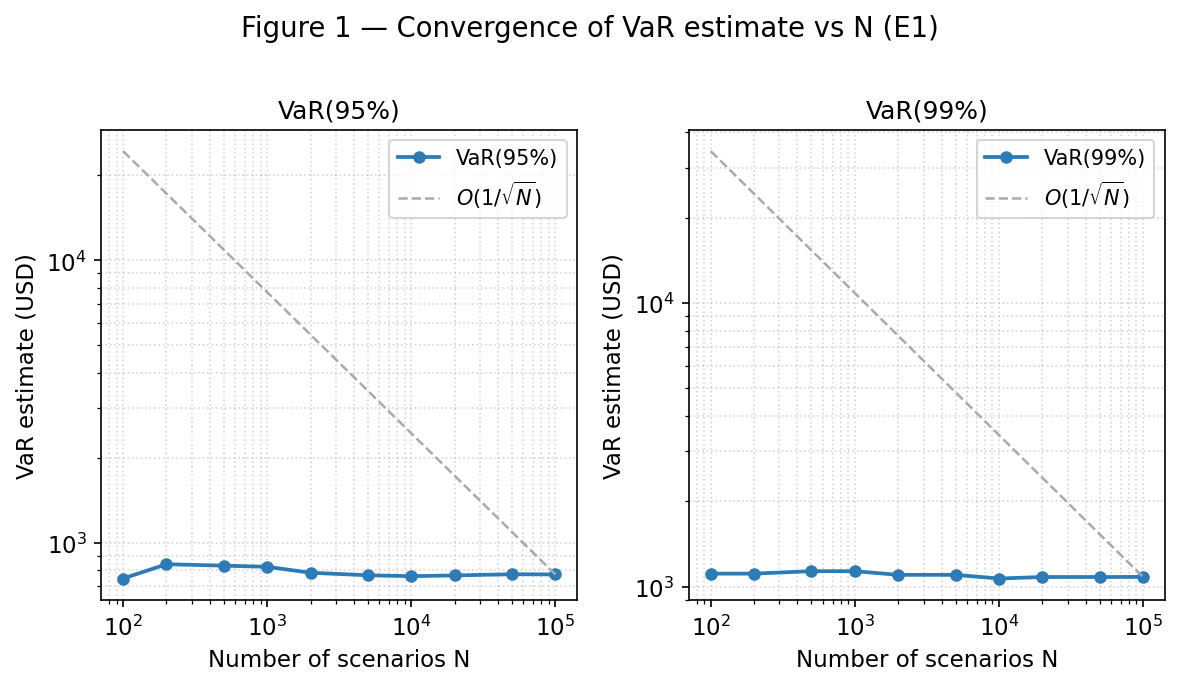
\includegraphics[width=\linewidth]{figures/fig1_convergence.png}
  \caption{VaR(95\%) and VaR(99\%) converge as $O(1/\sqrt{N})$.}
  \label{fig:convergence}
\end{figure}

Figure~\ref{fig:convergence} plots the bond-only VaR estimate from
$N = 100$ to $N = 100\,000$ scenarios.
Both VaR(95\%) and VaR(99\%) follow the $O(1/\sqrt{N})$
Monte Carlo convergence rate, validating the scenario generator and
the revaluation engine.  The deviation from the reference line at
small~$N$ reflects tail-sampling noise.

\subsection{E2 --- Stage timing (Dixon decomposition)}

\begin{figure}[h]
  \centering
  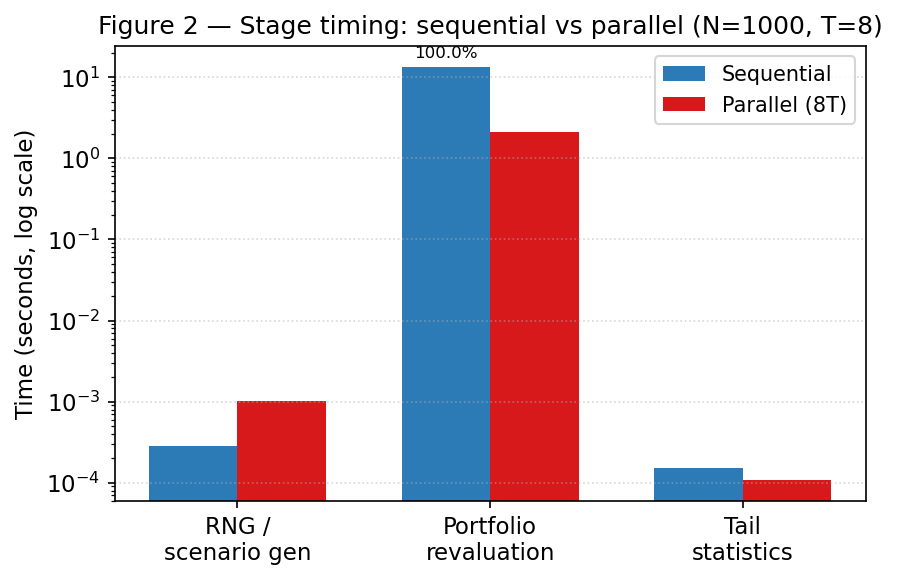
\includegraphics[width=\linewidth]{figures/fig2_stage_timing.png}
  \caption{Stage breakdown confirms revaluation dominates ($>$99.99\%).}
  \label{fig:stages}
\end{figure}

Following Dixon et al.~\cite{dixon2011}, we decompose runtime into
three stages.
Sequential ($N = 1\,000$): scenario generation 0.28\,ms (0.002\%),
portfolio revaluation 13.51\,s (99.997\%), tail statistics 0.15\,ms
(0.001\%).
Parallel 8-thread: revaluation 2.11\,s; the other two stages are
unchanged at sub-millisecond.
By Amdahl's law with a 0.003\% serial fraction, the theoretical
maximum speedup is $\approx 33\,000\times$, making this effectively
an embarrassingly parallel workload within the observed thread-count
range.

\subsection{E3 --- Strong scaling}

\begin{figure}[h]
  \centering
  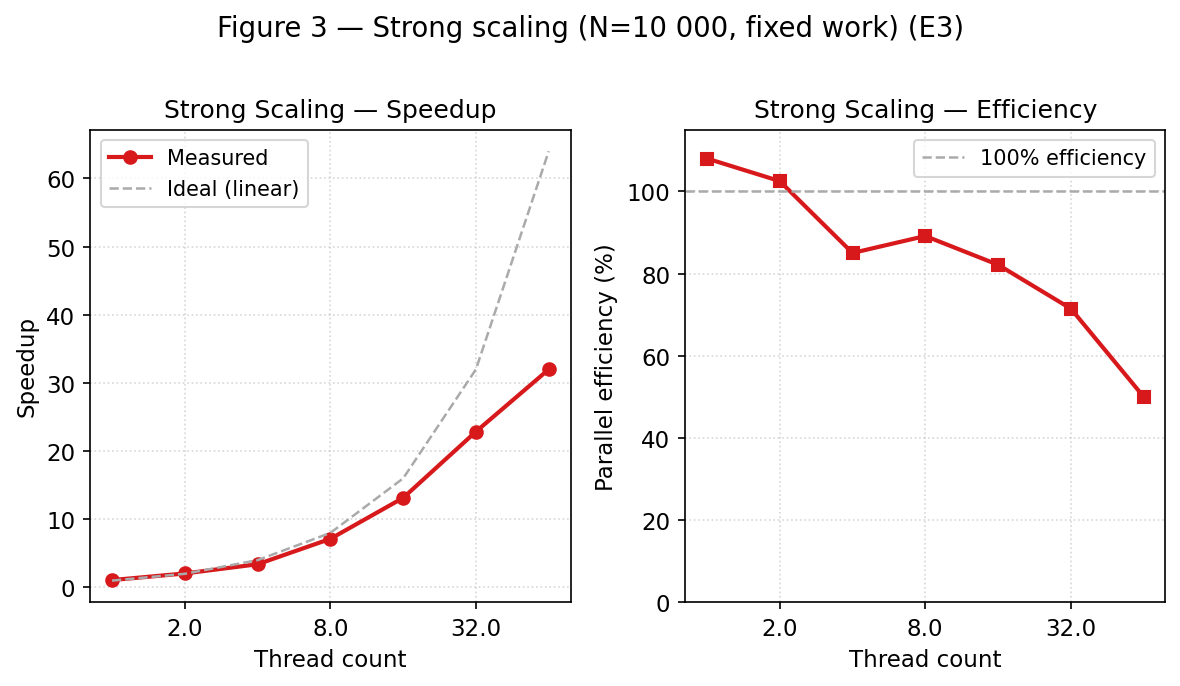
\includegraphics[width=\linewidth]{figures/fig3_strong_scaling.png}
  \caption{Strong scaling ($N = 10\,000$, fixed work).}
  \label{fig:strong}
\end{figure}

Figure~\ref{fig:strong} shows speedup and parallel efficiency
for $T = 1, 2, 4, 8, 16, 32, 64$ threads at fixed $N = 10\,000$
scenarios.  Results are summarised in Table~\ref{tab:strong}.

\begin{table}[h]
\centering\small
\caption{Strong scaling results.}
\label{tab:strong}
\begin{tabular}{rrrr}
\toprule
Threads & Wall (s) & Speedup & Efficiency \\
\midrule
seq & 126.1 & 1.00$\times$ & --- \\
1   & 116.9 & 1.08$\times$ & 100\% \\
2   & 61.5  & 2.05$\times$ & 100\% \\
4   & 37.1  & 3.40$\times$ & 85\%  \\
8   & 17.7  & \textbf{7.13}$\times$ & \textbf{89\%} \\
16  & 9.6   & 13.1$\times$ & 82\%  \\
32  & 5.5   & 22.9$\times$ & 71\%  \\
64  & 3.9   & 32.0$\times$ & 50\%  \\
\bottomrule
\end{tabular}
\end{table}

Scaling is near-linear through $T = 2$ and remains strong at $T = 8$
(89\% efficiency).
Degradation beyond $T = 16$ reflects cross-socket NUMA traffic:
each thread's independent market clone (curve, vol surface, 180
instruments) stresses the L3 cache and memory interconnect when
threads span more than one socket.
The efficiency drop from 82\% at $T = 16$ to 50\% at $T = 64$ is
consistent with the hardware topology (4 sockets at 16 cores each);
threads crossing a socket boundary pay an additional NUMA hop.

\subsection{E4 --- Weak scaling}

\begin{figure}[h]
  \centering
  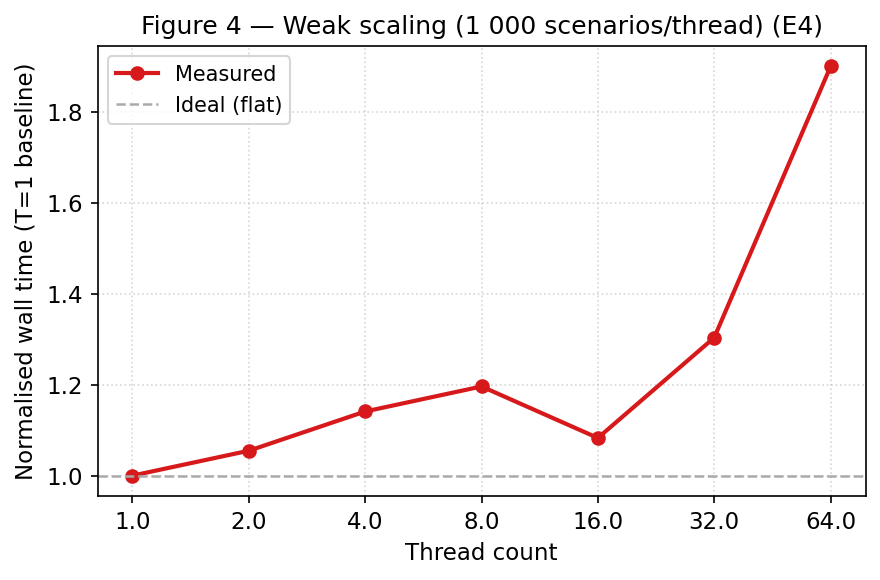
\includegraphics[width=\linewidth]{figures/fig4_weak_scaling.png}
  \caption{Weak scaling (1\,000 scenarios per thread).}
  \label{fig:weak}
\end{figure}

Figure~\ref{fig:weak} shows wall time normalised to $T = 1$ as
scenario count scales with thread count (1\,000 scenarios per thread).
Wall time rises by 20\% from $T = 1$ to $T = 8$, reflecting
OpenMP fork-join and per-thread context construction overhead.
The spike at $T = 64$ (+90\% over baseline) confirms that
the memory footprint of 64 independent portfolio clones
saturates aggregate NUMA memory bandwidth.

\subsection{E5 --- Schedule comparison}

\begin{figure}[h]
  \centering
  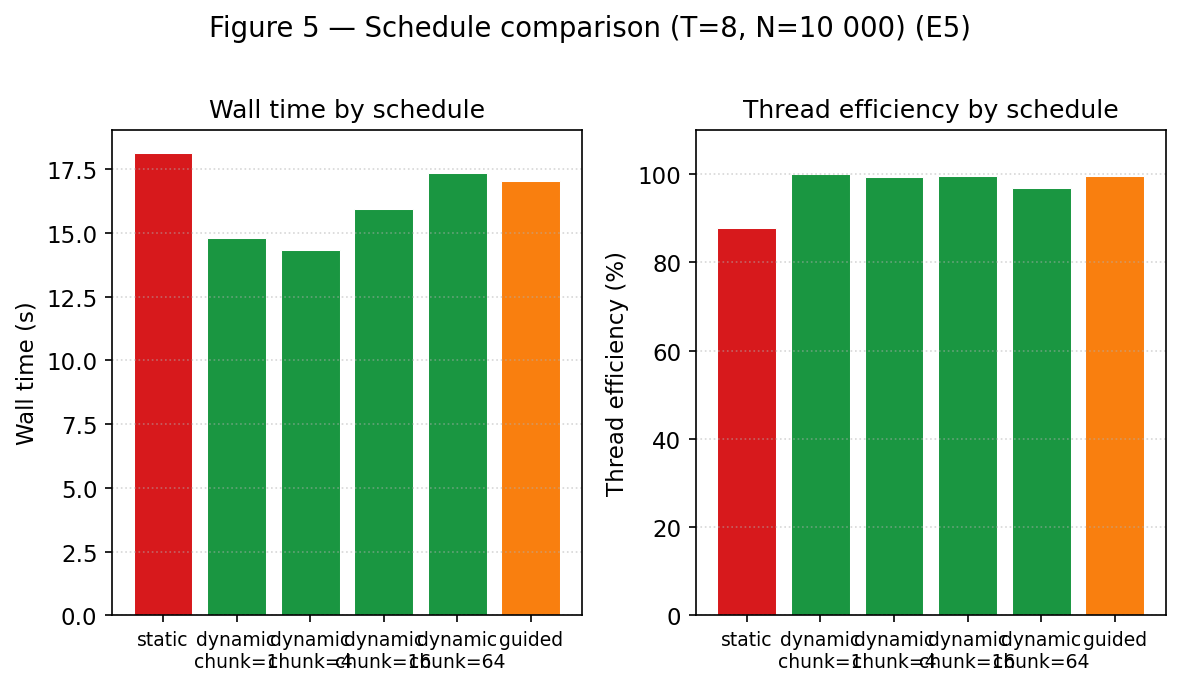
\includegraphics[width=\linewidth]{figures/fig5_schedule.png}
  \caption{Schedule comparison ($T = 8$, $N = 10\,000$).}
  \label{fig:schedule}
\end{figure}

Figure~\ref{fig:schedule} and Table~\ref{tab:schedule} compare
five scheduling configurations at $T = 8$ threads and $N = 10\,000$.

\begin{table}[h]
\centering\small
\caption{Schedule comparison ($T = 8$, $N = 10\,000$).}
\label{tab:schedule}
\begin{tabular}{llrr}
\toprule
Schedule & Chunk & Wall (s) & Thread eff. \\
\midrule
static   & ---  & 18.1 & 87.7\% \\
dynamic  & 1    & 14.8 & 99.9\% \\
dynamic  & 4    & \textbf{14.3} & 99.4\% \\
dynamic  & 16   & 15.9 & 99.5\% \\
dynamic  & 64   & 17.4 & 96.9\% \\
guided   & 16   & 17.0 & 99.5\% \\
\bottomrule
\end{tabular}
\end{table}

\texttt{schedule(static)} achieves only 87.7\% thread efficiency.
The 12.3\% idle time arises because the finite-difference American
option pricer's cost varies with scenario parameters: different
equity spot and vol values change option moneyness, which alters
the effective grid-convergence behaviour.  With static scheduling,
threads finishing their chunk early idle while slower threads
complete theirs.

\texttt{schedule(dynamic, 4)} is 21\% faster than static and
achieves 99.4\% efficiency.  Chunk size 4 amortises scheduler
overhead while remaining responsive to load variation; chunk 64 is
too coarse and approaches static behaviour.
This result validates Fusai et al.'s ``adaptive workload sizing''
recommendation for heterogeneous portfolios~\cite{fusai2006}.

\subsection{E6 --- Per-thread busy time}

\begin{figure}[h]
  \centering
  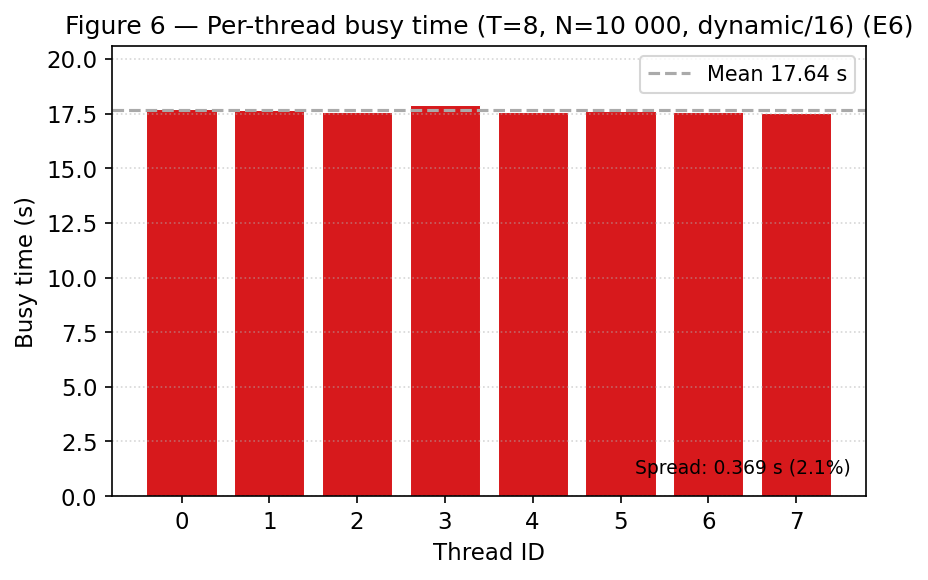
\includegraphics[width=\linewidth]{figures/fig6_thread_busy.png}
  \caption{Per-thread busy times ($T = 8$, dynamic/16).}
  \label{fig:busy}
\end{figure}

Figure~\ref{fig:busy} shows per-thread busy time accumulated via
\texttt{omp\_get\_wtime()} inside \texttt{ScenarioEvaluator::run()}.
All 8 threads remain busy for 17.55--17.91\,s (spread 0.36\,s,
2\% relative).  Near-perfect load balance at $T = 8$ confirms that
\texttt{schedule(dynamic)} distributes work evenly within a
single NUMA domain.

\subsection{E7 --- Cache and IPC behaviour}

\begin{figure}[h]
  \centering
  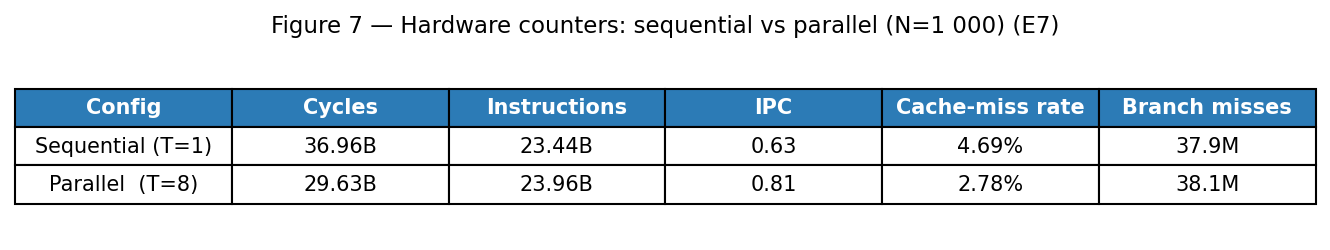
\includegraphics[width=\linewidth]{figures/fig7_cache_table.png}
  \caption{Hardware counters from \texttt{perf stat} ($N = 1\,000$).}
  \label{fig:cache}
\end{figure}

Sequential IPC of 0.63 indicates a memory-latency-bound workload:
the QuantLib observer pattern requires pointer chasing through
multiple heap-allocated objects per instrument reprice, creating
frequent L2/L3 misses (4.69\% miss rate).

Under 8-thread parallelism, IPC rises to 0.81 (+29\%) and the
miss rate drops to 2.78\%.  Both improvements arise from the
same mechanism: multiple independent instruction streams hide
memory latency by keeping the out-of-order execution units
occupied while cache fills are in flight.
Each thread's private market-data clone also fits better
in per-core L2 cache ($64\,\text{MiB}/\text{socket}$),
reducing cross-core evictions.

%% ============================================================
\section{Correctness}

Sequential and parallel engines produce \textbf{bit-identical}
P\&L vectors for the same seed across all thread counts and
schedule configurations tested (verified by byte-level diff of
output CSVs for $N = 1\,000$).
This holds because: (a) scenarios are pre-generated sequentially
so all threads read the same deterministic values; (b) each
\texttt{pnl[s]} slot is written by exactly one thread (no
reduction over shared state); (c) floating-point addition order
within a scenario is fixed (sequential inner loop over instruments).

The parametric VaR cross-check (bond-only subset, convexity-corrected)
passes within 10\% error.  The Black--Scholes spot check confirms
analytic European option prices match the \texttt{AnalyticEuropeanEngine}
to $< 10^{-6}$ absolute error.

%% ============================================================
\section{Conclusions}

We have demonstrated that the outer scenario loop of a Monte Carlo
VaR engine is an effective parallelization target on commodity
multicore hardware.  Key findings:

\begin{itemize}[noitemsep]
  \item \textbf{7.1$\times$} speedup at 8 threads (89\% efficiency);
    \textbf{32$\times$} at 64 threads.
  \item Portfolio revaluation accounts for 99.997\% of runtime
    (stage profiling, Dixon decomposition).
  \item \texttt{schedule(dynamic, 4)} outperforms \texttt{static}
    by 21\% due to scenario-dependent FD solver cost.
  \item Memory bandwidth (NUMA) is the binding constraint above
    $T = 16$; IPC improves from 0.63 to 0.81 under parallelism.
  \item All parallel results are bit-identical to the sequential
    baseline.
\end{itemize}

\paragraph{Future work.}
(1) \texttt{collapse(2)} over the (scenario $\times$ instrument)
space to expose intra-scenario load imbalance more sharply.
(2) Nested parallelism: outer scenarios $\times$ inner LSM MC paths
for American options.
(3) Philox counter-based RNG~\cite{salmon2011} for scalable
in-parallel scenario generation.
(4) Cholesky-correlated factor model~\cite{dixon2011,fusai2006}
to close the zero-correlation simplification.

%% ============================================================
\bibliographystyle{plain}
\bibliography{refs}

\end{document}
